% !TEX root = pfe-book3.tex
%!TEX TS-program = pdflatex
%!TEX encoding = UTF-8 Unicode


\cleardoublepage
%\mainmatter
\chapter{Electricity}
\label{ch-01}
%\thispagestyle{plain}
\section{Electric Current}

Using the study of electricity as an example, it is feasible (and necessary) to acquaint readers showing an interest in physics with the phenomenological approach to the investigation of nature. The word ``phenomenon'' from a Greek word meaning ``to appear'', is defined by the Webster Dictionary as ``any fact, circumstance, or experience that is apparent to the senses and that can be scientifically described or appraised''. The approach mentioned above, consists in the following. The investigator is not interested in the ``nature of things''. He uses words only to tell about facts. His aim is not to ``explain'', but only to describe phenomena. Almost all the terminology that he introduces is meaningful to him only if he can indicate some way to numerically evaluate the corresponding concepts.

He resorts to certain auxiliary names only to facilitate a verbal account of the facts. But the role of these names is absolutely secondary, they could just as well be replaced by other names or by simply saying ``something'' or ``thingumajig''.

The phenomenological method plays an immense role in natural science. Electrical phenomena are exceptionally suitable examples for explaining the essence of this method to the reader.

At the end of this chapter I shall review briefly the actual sequence of events in the history of electricity theory. At the present, I wish to present a certain idealized outline for the evolution of the phenomenological theory of electrical phenomena.

First, let us combine into a single mythical personage such scientists as Charles Augustin de Coulomb (1736-1806), Alessandro Volta (1745-1827), Georg Simon Ohm (1787-1854), Andre Marie Ampere (1775-1836), Hans Christian Oersted (1777-1851), Heinrich Friedrich Emil Lenz\footnote{Known as Emil Christianovich Lenz in his native Russia.} (1804-1865) and others of that ilk. Imagine that our corporate investigator is endowed with a capacity for modern scientific thought, and let us equip him with a complete set of up-to-date terminology. This composite scientist is to play the chief role in our further discussion.

He begins to conceive a phenomenological theory of
electricity by carefully examining a storage battery. The first feature he takes notice of is that the battery has two ``poles''. Touching them with his two hands, he instantly learns that this is something to avoid (the shock may be quite severe). But after this first experiment, it probably occurs to him that something passed through his body; we shall name this ``something'' electricity. Being extremely careful not to suffer another shock, be begins to connect the poles (actually terminals) by various wires, rods and cords. He then discovers the following: of the articles brought into contact with the two poles, some are intensely heated, others become only warm and, in some cases, no heating is observed. 

Selecting appropriate words to describe his discovery, our investigator decides to speak of it as follows: ``When I connect the poles with a wire, electricity flows through the wire. I shall call this phenomenon an electric current. Experiments indicated that items of different materials are differently heated by the current. Those which are only slightly heated evidently ``conduct'' electricity poorly or offer high resistance to the current. They can be called \emph{insulators} or \emph{dielectrics}.''

Next our investigator begins experimenting with liquids. Again he finds that different substances behave differently. Finally, he makes an interesting discovery: taking a solution of copper sulphate and immersing carbon electrodes (as we call the items connected to the poles) into the bath, our scientist finds a reddish copper deposit on one of the carbons.

At this stage, our investigator becomes convinced that the phenomenon he is studying has to do with the flow of some kind of fluid. It obviously makes sense to speak of the direction of flow. Let us agree upon marking the electrode on which the copper is deposited with a minus sign and consider the other electrode to be positive. Since it is longish and inconvenient to say ``negative electrode'' and ``positive electrode'' each time, the terms \emph{cathode} and \emph{anode} are suggested instead. Current passage is from the plus to the minus, i.e. from the anode to the cathode.

But the value of the discovery is far from being exhausted at this point. It is further established that an equal mass of copper is deposited on the cathode each second. Evidently, the copper atoms carry the electric fluid. Therefore, the investigator introduces two new terms. First, he supposes that the mass $M$ of the copper is proportional to the quantity $q$ of electricity flowing through the circuit, i.e. he introduces the equation
\begin{equation*}%
q = kM
\end{equation*}
where $k$ is the proportionality factor. Next, he proposes that the quantity of electricity passing along the circuit in unit time be called the \emph{current strength} or, simply, \emph{current}:
\begin{equation*}%
I = \frac{q}{\tau}
\end{equation*}
Our investigator has become substantially enriched. He can now characterize the current by two measurable quantities: by the amount of heat evolved by a definite portion of the circuit in unit time; and by the current, the quantity of electricity flowing in unit time.

This leads to a new opportunity: he can compare the currents produced by various sources. He measures the current $I$ and then the energy $Q$ generated in the form of heat, by a single piece of wire. Repeating the experiment with various conductors, the investigator finds that the ratio of the amount of heat generated to the current in the wire differs for various current sources. It remains to invent a term for this ratio. It was called the \emph{voltage}. The higher the voltage, the more the heat generated.

This last statement can, to some small extent, justify our choice of terms. The more the tension required to pull a loaded wagon (and tension is sometimes used to denote voltage, e.g. high-tension current), the hotter we get. Denoting the voltage by $V$, as is customary today, we obtain
\begin{equation*}%
V = \frac{Q}{q}, \,\, \textrm{or} \,\, Q = V I \tau
\end{equation*}
Thus, the first steps have been taken. Two phenomena have been discovered. An electric current deposits matter in passing through certain liquids, and an electric current generates heat. Heat is something we are capable of measuring. The method for measuring the quantity of electricity has been devised, i.e. a \emph{definition of this concept has been given}. Definitions have also been given for \emph{derived} concepts: the current and the voltage.

A number of simple equations have been written, but notice that they cannot be called laws of nature. For instance, our investigator \emph{called} the ratio $Q/q$ the voltage, instead of \emph{finding} that $Q/q$ is equal to the voltage.

Now, he begins to search for the law of nature. Two quantities can be measured for the same conductor: the current and heat evolved, or the: current and voltage (which, in principle, mean the same).

An investigation of the dependence of the current on the voltage leads to the discovery of an important law. The vast majority of conductors comply with the law:
\begin{equation*}%
V=IR
\end{equation*}
The quantity $R$ can be called the resistance; this fully agrees with the initial qualitative observations. The reader has, of course, recognized this equation; it is \emph{Ohm's law}. Substituting the value of the current from Ohm's law into our preceding formula, we obtain
\begin{equation*}%
Q = \frac{V^{2}}{R} \tau
\end{equation*}
You will not be confused, I hope, by the possibility of writing the expression for the energy evolved by a conductor in the form of heat in a different way:
\begin{equation*}%
Q = I^{2}R \tau
\end{equation*}
It follows from the first of the last two formulas that the amount of heat is inversely proportional to the resistance: This is true if we add at constant voltage. This is the case we had in mind when we first used the term ``resistance''. The second formula, contending that the heat is directly proportional to the resistance, requires the condition: at constant current.

These two equations are evidently recognized by the reader as the law named after James Prescott Joule (1818--889) and Lenz (the \emph{Joule-Lenz law}).

Finding thus that the voltage and current are proportional, thereby enabling the resistance of a conductor to be determined, our investigator naturally poses the question: How is this important quantity related to the shape and size of the conductor and to the material of which it is made?

Experiments lead to the following discovery. It is found that
\begin{equation*}%
R = \rho \frac{l}{A}
\end{equation*}
where $l$ is the length of the conductor and $A$ is its cross-sectional area. This simple equation is valid when we deal with a linear conductor of constant cross section along its whole length. Resorting, if necessary, to more complex mathematical operations, we can write the resistance formula for a conductor of any shape. What, here, is the factor $\rho$? It characterizes the material of which the conductor is made. The value of this quantity, named the \emph{resistivity}, varies in an extremely wide range. The resistivity of various substances may vary by thousands of millions of times.

Let us carry out several formal transformations that will prove useful further on. Ohm's law can be written as
\begin{equation*}%
I = \frac{VA}{\rho l}
\end{equation*}
A frequently employed quantity is the ratio of the current to the cross-sectional area of the conductor. It is called the \emph{current density} and is usually denoted by the letter $j$. Then the same law can be written as
\begin{equation*}%
j = \frac{1}{\rho} \frac{V}{l}
\label{curr-density}
\end{equation*}
At this point, it seems to our investigator that he has found everything related to Ohm's law. If he has at his disposal an unlimited number of conductors of known resistance, our investigator can reject the cumbersome technique of determining voltage by means of a calorimeter: he now knows that the voltage equals the product of the current by the resistance.

Our investigator soon finds, however, that this statement is in need of refinement. Using the same current source, he connects its poles through various resistances. The current naturally differs in each experiment. But, he finds, the product $IR$ of the current and resistance does not remain constant. When he studies this, as yet unexplained, phenomenon, the investigator finds that with an increase in the resistance the product $IR$ tends to a certain constant value.

Denoting this limit by $\mathcal{E}$, we derive a formula that does not coincide with the one established when measuring the voltage and current. The new formula is
\begin{equation*}%
\mathcal{E} = I (R + r)
\end{equation*}
What a strange contradiction!

After some thinking, we come to the conclusion that there is, of course, no real contradiction. When we directly measured the voltage with a calorimeter, we were concerned only with the conductor that connected the storage battery terminals. It must be clear, however, that heat is also evolved in the battery itself (we can make sure by touching the battery with our fingers). The storage battery has its own resistance. The meaning of quantity r, found in the new formula, is obvious, it is the internal resistance of the current source. Quantity $\mathcal{E}$ requires a special name. One cannot contend that the name selected is particularly appropriate. Quantity $\mathcal{E}$ is called the \emph{electromotive force (emf)}, though it has neither the meaning nor the dimensionality of force.

Both formulas continue to be called Ohm's law (observing, so to speak, historical fairness), only the first is called Ohm's law for a portion of a circuit, and the second, Ohms law for the  whole circuit.

Now, everything seems to be cleared up. The laws of direct current have been established.

But our investigator is still unsatisfied. Even without direct measurement of the voltage with a calorimeter, its determination remains cumbersome. Imagine weighing the cathode with its copper deposit each time! You must admit that this is extremely inconvenient, to say the least.

One truly fine day, our investigator quite accidentally placed a compass near a conductor in which there was a current. This turned out to be a great discovery. The magnetic needle turned violently when current passed through the, conductor, turning in the opposite direction when the current was reversed.

The moment of force acting on the magnetic needle can be readily determined. Hence, a measuring instrument can be devised on the basis of this observed phenomenon. All that is required is to establish the dependence of the moment on the current. Our investigator solves this problem and designs excellent pointer-type instruments for measuring the current and voltage.

Our account of the research carried out by our composite investigator during the first half of the nineteenth century in studying the laws of direct currents would not be complete if we did not mention that he discovered the interaction of currents. Parallel conductors with currents travelling in the same direction attract each other. They repel each other when the currents travel in opposite directions. Of course, this phenomenon can also be used to measure the current.

I shall certainly not limit myself to the last paragraphs in presenting the laws of electromagnetism; a whole chapter is devoted to this subject. But I had to remind the reader of these important facts to achieve the aim of the present chapter, which is to show how the basic quantitative concepts and units of measurement describing electrical phenomena -- current, charge and field -- are introduced.

\section{Stationary Electricity}

We shall assume that our idealized investigator has a comprehensive knowledge of the wide variety of phenomena that were said to be electrical in the remote past. The special properties of amber, or a glass rod rubbed with fur, the initiation of sparks jumping between two bodies that have been electrified were studied (or, rather, were used for striking demonstrations) for a sufficiently long time. Naturally, our investigator studying electric currents asked himself: Is the fluid passing through a wire and the one that can exist in a stationary state on some body until the body is ``discharged'' one and the same ``something''?

Even if we digress from the information that has been accumulated previously, is it not necessary to pose the question: If electricity is ``something'' that flows through a conductor like a liquid, can it be ``poured into a glass''?

If our investigator wants a direct answer to this question, he should proceed as follows. First he obtains a current source of sufficiently high voltage (so far we have not mentioned units of measurement, and so the reader should wait a while before asking what we mean by a high voltage, a heavy current, etc.). One of the battery poles is grounded and a tiny hollow bead, made of very thin aluminium foil, is placed on the second pole. This bead is suspended by a silk thread. The same is done with another such bead.

Next the two tiny beads are brought close together (say, to a distance of \SI{2}{\milli\meter} between their centres).

To his extreme delight or amazement (or any other epithet you care to use), our investigator finds that the beads repel each other. From the angle between the threads and the known mass of the beads, he can compute the force acting between the beads.

The investigator also establishes the following fact: if the beads are charged by touching the same pole of the battery, they repel each other. If one bead obtains electricity from one pole and the other bead from the other pole, they attract each other.

This experiment confirms the right to speak of electricity as something behaving like a liquid and shows that we can deal both with electricity in motion and at rest.

Since our investigator can determine the quantity of electricity by weighing the mass of the copper deposited on the cathode, he can find ``how much liquid was poured into the glass'', i.e. the quantity of electricity taken by the bead from the battery electrode.

First of all, the investigator observes the following. If a charged bead is earthed, or grounded, i.e. connected to the earth by a wire or other conductor, the bead loses its charge. Next, he can show that the charge ``drains'' through the wire, i.e, that a current passes through the wire. Finally, he can measure the amount of copper deposited on a cathode in an instrument with an electrolyte (conducting solution), inserted into the path of the charge to the earth. This, in other words, is a measurement of the quantity of static (stationary) electricity that was on the charged bead.

This quantity of electricity is called the \emph{charge} on the bead by our investigator who ascribes a sign -- $(+)$ positive or $(-)$ negative -- depending upon which electrode the electric fluid was taken from.

Now we can commence our next series of experiments. Various quantities of electricity can be obtained by beads or balls of various sizes from the poles of various batteries. Locating the balls at different distances from one another, he can measure the force of interaction between them. This leads him to the following important law of nature:
\begin{equation*}%
F = K \frac{q_{1}q_{2}}{r^{2}}
\end{equation*}
which states that the force of interaction is directly proportional to the product of the charges on the balls and inversely proportional to the square of the distance between them. The reader recognizes it as the expression of \emph{Coulomb's law} which was established differently than we have described. But our investigator is no historical character.

Our investigator knows of forces of two different kinds. One kind is developed upon direct contact of one body with another. Such is the case in pulling or pushing. With respect to forces that act at a distance, so far he knew only of the force of gravity or, in a wider aspect, the force of universal gravitation.

Thus a new force was added to the remotely acting ones: the force of Coulomb attraction or repulsion between two charged bodies. It closely resembles the gravitational force. Even the formulas resemble each other.

The force of gravity exerted by the earth on a body does not lead to any particular difficulties in calculations. As for Coulomb, or, as they are also called, electrostatic, forces, we may encounter cases in which electric charges are distributed in space in some complex and, even worse, unknown manner.

But we can manage without knowing the way in which the charges are distributed. We know that these charges ``sense'' one another at a distance. Why not say that the charges set up an \emph{electric field}? It may seem at first that difficulties arise from the fact that we cannot see the electric field. ``But I think,'' says our investigator, ``that the electric field should not be regarded as mathematical fiction for facilitating calculations. If a charge located at some point is subject to a force, this means that this point (in space) is in a special state. An electric field is a physical reality, i.e. it exists by itself even though we cannot see it.'' Since he made this guess at the beginning of the nineteenth century, our investigator could not prove it. But the future showed that it was correct.

Coulomb's law establishes a formula by means of which we can determine the effect of one small ball on another. One of the balls can be fixed and the other moved to various points in space. At all points the movable (test) ball is subject to a force. Today, this fact is differently formulated: a ball charged with electricity sets up a field of electric forces or, more concisely, an electric field about itself.

The source of an electric field may be charged bodies of any shape. Coulomb's law is not valid in this case, but, using a test ball, we can measure the electric field surrounding a charged body and specify this field in an entirely comprehensive way by indicating the magnitude and direction of the forces. To avoid the dependence of the specification of an electric field on the charge of the test ball, an electric field is characterized by its intensity:
\begin{equation*}%
E = \frac{F}{q}
\end{equation*}
where $q$ is the electric charge of the test ball.

There is a visual way of describing an electric field by lines of force. Diagrams showing these lines of force may differ greatly depending upon the shape of the charged bodies and their mutual location. The simplest diagrams of electric fields are illustrated in \figr{fig-1.1}. Their meanings are the following. A tangent at any point to a line of force indicates the direction of the electric force at that point. The number of lines per unit of area perpendicular to the lines of force is entirely arbitrary provided that it is proportional to quantity $E$. When, however, we speak of the number of lines of force without using a diagram, it is assumed that this number is simply equal to $E$.
\begin{figure}[!ht]
\centering
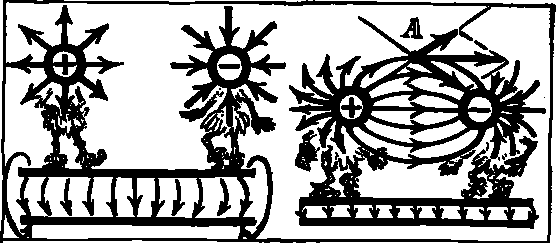
\includegraphics[width=\textwidth]{figures/fig-01-01.pdf}
\caption{Electric field lines from a charged body.}
\label{fig-1.1}
\end{figure}

If a free electric charge is placed in an electric field, it moves along the lines of force, unless other forces, for instance gravity, interfere.

Of simplest appearance are force fields set up by bodies of spherical shape. If two spheres or two charges that can be regarded as points approach each other, their fields are superimposed. Their field intensities are added by the parallelogram method. We can determine the direction of the line of force at any point $A$ and find the field intensity by constructing the parallelogram of forces as shown in \figr{fig-1.1}.

If the charged bodies are in the form of plates, the field resembles that shown at the bottom of \figr{fig-1.1}. By bringing the plates closer together and increasing their area, we can obtain almost ideal field uniformity, with only a slight edge, or fringe, effect. It can be said of two closely located plates that they condense the field. Accordingly, such a device is called a condenser. It is now generally known as a capacitor.

As we know, work done in moving a body subject to a force is equal to the product of the force by the length of path. To transfer a charge from one plate of a capacitor to the other along a line of force, the work required is equal to $qEl$. The work required to carryover a unit quantity of electricity equals $El$.

Now let us connect the two plates of a capacitor with a conductor. The amount of energy generated when quantity $q$ of electricity is passed through the conductor equals $qV$. Since we already realize that there is no difference in principle between the motion of a charged ball in an electric field and the passage of the electric ``fluid'' along the metal conductor, we can equate these two expressions for the energy expended by the field. Thus
\begin{equation*}%
qEl = qV
\label{energy-field}
\end{equation*}
The validity of this equation can be readily checked by moving the plates of a capacitor farther apart and measuring the force exerted on a test charge.

This measurement can be done by an elegant procedure without resorting to a charged ball suspended by a silk thread.

Everybody knows that light bodies fall considerably slower than heavy ones. It will be recalled that this is what led wise men of antiquity and the Middle Ages to suppose, previous to Galileo's experiments, that the velocity of motion (and not the acceleration) of a body is proportional to the force acting on it. This point of view was proved false only after it had been demonstrated that a piece of paper and a metal ball drop side by side in a vertical glass tube from which the air has been pumped out. It was found that all bodies gain velocity in falling at the same rate, i.e. fall to the earth with the same acceleration. For our purposes, however, we can utilize the influence of air resistance to make our light hollow metal ball (or bead), used to demonstrate Coulomb's law, fall very slowly.

If this ball is dropped between the plates of a capacitor, we can vary the voltage between the plates until the electric field that is set up stops the ball from falling further. Equilibrium is achieved when the force of gravity equals the field force: $mg = qE$. This equation can be used to determine the field intensity and to prove the validity of our theoretical reasoning.

The number of lines of force passing through any imaginary or real surface in an electric field is selected so that in our chosen units of measurement it equals the electric flux. Can we find the electric flux passing through a closed surface that encompasses charged bodies?

Let us first consider the simplest case. The field is set up by one small ball. We describe a sphere around the ball. If the radius of the sphere is $R$, then the intensity at any point of the surface on the sphere is $Kq/R^{2}$. The area of the sphere is $4\pi R^{2}$. Thus the electric flux through the sphere is $4 \pi Kq$. It is clear, however, that the flux remains the same regardless of the kind of surface we consider.

Next we complicate the picture by assuming that the field is set up by a large number of charged bodies of any shape. These bodies, however, can be imagined to be broken down into tiny portions, each being equivalent to a point charge. We enclose the system of charges with a surface of arbitrary shape. The flux from each charge equals $4 \pi Kq$. It is quite natural to assume that the fluxes can be added together arithmetically. Hence, the total flux through any closed surface, encompassing all the charges, is proportional to the sum of the charges of all the bodies enclosed in this surface.

This statement is the basic law governing electric fields (one of Maxwell's four equations, see \hlgray{Chapter \ref{ch-05}}). 

Note that we neither derived nor proved this formula. We simply guessed that this is the way things are and not differently. This means we are dealing with a general law of nature whose validity is established by an experimental confirmation of any consequences that follow from the general law.

It is vitally important to know the general rule that holds for any system. On the basis of the written law, an electronic computer requires only seconds to calculate the required data on an electric field set up by a most complex system of charged bodies. We shall restrict ourselves to the modest problem of deriving a formula of practical importance for determining the capacitance of a capacitor (demonstrating, at the same time, techniques of theoretical physics applied to an elementary case).

First we define this well-known quantity. The capacitance of a capacitor is the ratio of the charge that accumulates on its plates to the voltage applied across the plates. Thus
\begin{equation*}%
C  = \frac{q}{V}
\end{equation*}
In a capacitor, the lines of force do not pass out beyond the edges of the plates to any appreciable extent. They emerge from the positive plate and enter the negative one. Neglecting distortion of the field at the edges of the capacitor, we can write the product $EA$ for the flux. It follows from the general law that
\begin{equation*}%
EA = 4 \pi K q
\end{equation*}
from which the field intensity between the plates is
\begin{equation*}%
E  = 4 \pi K \frac{q}{A}
\end{equation*}
On the other hand, the field intensity of a capacitor can
be written as
\begin{equation*}%
E  = \frac{V}{d}
\end{equation*}
where $d$ is the distance between the plates. Equating the last two equations and recalling that $C=q/V$, we obtain the formula for the capacitance of a capacitor:
\begin{equation*}%
C  = \frac{A}{4 \pi Kd}
\end{equation*}
In their actual design, capacitors are strips of metal pressed against the faces of strips of mica or paraffin-impregnated paper. The last two are insulating materials. What do we gain by inserting a dielectric between the capacitor plates? Experiments show that the capacitance $C$ of a capacitor is related to its capacitance $C_{0}$ when it has no separating medium by the formula $C=C_{0}\varepsilon$.

The constant $\varepsilon$ is called the \emph{permittivity}, or \emph{dielectric constant}. For air, mica, water and Rochelle salt, the permittivities are equal to 1, approximately 6, 81 and 9000.

\section{What Is Basic?}

Ohm's law and the Joule-Lenz law relate energy, current, voltage and resistance. We can say that the voltage is equal to the product of the current by the resistance. But we can also say: the current is the voltage divided by the resistance. Both definitions are found in textbooks and both have the shortcoming that they
prove convenient only in cases when Ohm's law is valid. And, as mentioned before, this law is not always true. Consequently, it is better to proceed as we did, namely, to assume that the derived quantity is the resistance of the conductor, and that it is defined as the ratio of the voltage across the ends of the conductor to the current passing through it.

Since the energy of an electric current can be measured on the basis of the energy conservation law -- by the thermal or mechanical effects of the current -- it is clearly expedient to define the current or voltage as quantities derived from the energy. The most natural procedure is to determine the current from electrolysis phenomena and the voltage across the ends of a portion of a circuit as the quotient of the generated energy divided by the quantity of electricity.

The reader must clearly perceive, however, that this is not the only possible system of determining these electrical quantities. Instead of electrolysis, i.e. deposition of metal on an electrode, the current can be determined on the basis of any other of its effects, such as the effect of a current on a magnetic needle or on another current.

There is nothing wrong in principle with another procedure: we select a certain standard current source and then the voltage of any other current source is determined as the number of equal standard elements. Such a proposal was made, and the standard element is called the Weston cell.

Still another possibility is to devise the system of definitions and units of measurement by selecting a certain standard resistance. Then, as above, we find how many standard resistances can substitute for the given conductor. At one time, a column of mercury of specified length and cross section was used as such a unit of resistance.

It is helpful to understand that the sequence in which physical concepts are introduced is a random matter. It does not in any way, of course, alter the laws of nature.

So far we have dealt with phenomena concerned with direct electric current. Even within this group of phenomena it is feasible to devise various systems of concepts and, consequently, various systems of units of measurement. Actually our choice is even more extensive because electrical phenomena are not at all restricted to those dealing with direct electric current.

Many physics textbooks, including ones recently published, define the concept of the quantity of electric charge (or the quantity of electricity, which is the same thing) from Coulomb's law. Then the textbooks treat of voltage and only later, after finishing the discussion of electrostatics, do they introduce the concepts of the current and electrical resistance. As you have seen, we went about this matter in a different way.

There is even more freedom in selecting the units of measurement. The investigator has the right to proceed as he finds convenient. He should never forget, however, that the selection of the units of measurement affects the proportionality factors he must use in various formulas.

There is nothing wrong (again, in principle) with selecting the units of current, voltage and resistance independently of one another. But this requires introducing into Ohm's law a factor with specified dimensions. Until quite recently, before the habitually familiar calorie had been banished forever from physics by a stern international committee, the formula of the Joule-Lenz law had a numerical factor. This was due to the fact that the units of measurement for current and voltage were defined quite independently of the selected units for energy (heat and work).

In the preceding paragraphs, I have written only two formulas in the form of proportionalities, all the rest are equations without numerical coefficients. One of these two formulas relates the mass of the substance deposited on the electrode with the quantity of electricity, and the other is Coulomb's law. This was not done by accident, but because physicists seem to be unwilling, so far and to some extent, to go over to the International System of Units, SI, accepted as a law, and continue to employ the absolute physical system (cgs units) in their work (less and less, it is true, due to the pressure exerted on them by the editors of their articles and books). In the absolute physical system, the quantity $K$ in the Coulomb formula for the interaction of charges in a vacuum is set equal to unity. When this is done, the value of the so-called ``absolute'' unit of the quantity of electricity is predetermined (the charge equals unity if two identical charges, located at unit distance from each other, interact with unit force).

After measuring the mass in grams, it would be necessary, to remain consistent, to calculate the value of factor $k$ in the law of electrolysis, indicating how much matter is deposited on the electrode in the passage of one absolute unit of charge. But it is of no avail to look through your textbooks in search of such a value of this factor. Knowing the obstinate reluctance of engineers to reject the ampere and coulomb, physicists made use in the law of electrolysis of a number indicating the mass of matter deposited when one coulomb of electricity passes through the electrolyte. Thus, two units were given in books for the same quantity. It was also clear that it was convenient to employ one or the other in entirely different cases, because the coulomb is equal to three thousand million absolute units.

It is convenient, of course, to have $K$ equal to unity, but engineers drew attention to the fact that formulas for the electric flux, capacitance of a capacitor and others include the unwanted coefficient $4\pi$. They contended that it would be a good thing to eliminate it.

As is usual in such controversies, victory was celebrated by those closer to practice than to theory. The system accepted today proceeded along the course that engineering has long followed. Supporters of the SI system insisted on using a single unit of energy in all branches of science and also required that the current, or current intensity, be accepted as the only basic electrical concept.

Thus, we begin the study of electricity with the \emph{joule} as the unit of energy. We select the \emph{coulomb}, equal to the ampere-second, as the unit of the quantity of electricity. We propose that the ampere be defined from the force of interaction of currents. This definition (given on page \pageref{ampere-def} in the chapter devoted to electromagnetism) is devised so that factor $k$ in the electrolysis formula remains the same one that everybody has long become accustomed to. Still, we must understand that in the SI system of units this factor \emph{does not determine} the value of the coulomb. With the increase in the accuracy of measurement, we will be obliged to revise this value so as to retain the definition of the ampere (I do not think such a time will come, because I cannot conceive that the measurement of electrodynamic forces can be more precise than the measurement of mass).

The SI system next follows the course I plotted for our composite investigator. First came the unit of voltage, called the \emph{volt}, equal to one joule divided by one coulomb; then the unit of resistance, called the \emph{ohm}, equal to one volt divided by one ampere; the unit of resistivity, one ohm multiplied by one metre, etc.

Now we have reached Coulomb's law and find that we no longer have the right to dispose of factor $K$. The force is measured in newtons, the distance in metres and the charge in coulombs. Factor $K$ acquires dimensionality and has a certain value determined experimentally.

Coulomb's law is rarely required and the equation for the capacitance of a capacitor is the working formula in many engineering calculations. To eliminate factor $4\pi$ in formulas for the electric flux, capacitance of a capacitor and others, engineers replaced factor $K$ by the expression $1/4\pi \varepsilon_{0}$ a long time ago. For readily understandable reasons, the quantity $\varepsilon_{0}$ can be called the \emph{electrical permittivity of vacuum}. It equals
\begin{equation*}%
\varepsilon_{0} = \num{8.85d-12} \frac{\textrm{coulomb}^{2}}{\textrm{newton-meter}^{2}}
\end{equation*}
Hence, the flux of lines of force is expressed by

\begin{equation*}%
\frac{1}{\varepsilon_{0}}(q_{1} + q_{2} + \ldots)
\end{equation*}
and the capacitance of a capacitor is written as
\begin{equation*}%
C = \frac{\varepsilon\varepsilon_{0}A}{d}
\end{equation*}
The unit of capacitance, one \emph{farad}, equals one coulomb divided by one volt.

\section{Evolution of Electricity Theory}
The actual evolution of electricity theory was not at all along the lines followed by our mythical composite investigator.

Electrostatic phenomena were well known in ancient times. It is difficult to say today whether the ancient Greeks knew what bodies in addition to amber (the Greek word for amber, \emph{elektron}, is the source of such words as electricity, electron, etc.) acquire special properties after being rubbed and attract small bits of straw. Not until the beginning of the $17^{\textrm{th}}$ century did Sir William Gilbert (1540-1603) show that this strange property was possessed by diamond, sealing wax, sulphur, alum and many other substances. This outstanding English physicist, who was also court physician to Queen Elizabeth I, was evidently the first to devise instruments that could be used to observe the interaction of electrified bodies. By the $18^{\textrm{th}}$ century it was already known that certain bodies are capable of retaining charges, while the charges ``leak away'' from other bodies. Few scientists of this century doubted that electricity was something resembling a fluid. The first electrostatic machines were built. They produced sparks and could ``shock'' a line of people holding hands when one of the end persons touched a terminal of an operating electrostatic machine. It was considered good taste for the courts of many countries to visit the laboratory of a scientist as they would go to a circus. And the scientists, in their turn, made every effort to dramatize the phenomena being demonstrated.

In the $18^{\textrm{th}}$ century we can already speak of electrostatics as a science. A great many different kinds of electroscopes were invented and made; Coulomb began his quantitative measurements of the interaction forces between charges.

In 1773, the Italian physician and physicist Luigi Galvani (1737-1798) began to investigate the contraction of the leg muscles of a dead frog when a voltage was applied across them.

Continuing Galvani's experiments, Volta came to the Conclusion at the end of the $18^{\textrm{th}}$ century that an electric fluid passed through the frog's muscles. The next remarkable step forward was the invention of the first current source, the galvanic cell, and later, the voltaic pile.

At the very beginning of the $19^{\textrm{th}}$ century, Volta's discoveries were known by the whole world of science. This started off extensive investigations of electric current. New discoveries followed, one after the other.

A number of investigators studied the thermal effects of current. This is what Oersted was engaged in when, entirely by chance, he discovered the effect of a current on a magnetic needle.

The brilliant investigations of Ohm and Amp\`ere were conducted at about the same time: in the twenties of the nineteenth century.

Amp\`ere's work quickly won him worldwide fame. Ohm had no such luck. His scientific articles, combining neat and elegant experiments with precise calculations, distinguished by their rigorous substantiation and systematic introduction of phenomenological concepts, paying absolutely no attention to the ``nature'' of things, were not appreciated by his contemporaries. When anyone mentioned Ohm's works, it was only to ridicule the ``morbid fantasy of the author, who is trying to belittle the dignity of nature''. (These words belong, evidently, to the physicist De la Rive, who made no contribution whatsoever to science.)

It is extremely difficult to read the original works of physicists written in those days. Experimental discoveries were described in language alien to us today. It is even impossible, in many cases, to understand what the author meant by certain words. The names of famous scientists are retained in the memory of posterity only due to the efforts of historians of science.





